
The following section will introduce the software segment, based on the required specifications. The design will be shown in the form of a flowchart.
The section consists of the PID controller and the Pulse width modulator as well as showing the ADC initialization.

\subsection{Software diagram}

\begin{figure}[h!]
  \centering
  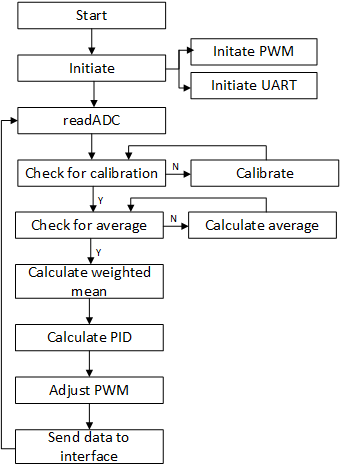
\includegraphics[width=0.6\textwidth]{figures/softwareflowchart.png}  
\caption{Software flowchart}  
  \label{Softwareflowchart}
\end{figure}

\newpage
\section{Analog to digital conversion}


\begin{lstlisting}
extern int analogRead(char CH) {
    AD1PCFG = ~CH;
    AD1CON1 = 0x0000; //AMP bit = 0 ends sampling and starts converting
    AD1CSSL = 0; //Input scan select, not used
    AD1CON3 = 0x0001; //Manual Sample, TAD = internal 4 TPB
    AD1CON2 = 0; //No scanning, interrupt at completion of each sample, one 16-word buffer
    AD1CON1SET = 0x8000; //Turn on the ADC
    AD1CHSbits.CH0SA = CH;
    AD1CON1SET = 0x0002; //Start sampling
    DelayUs(2); //Wait 2 microseconds
    AD1CON1CLR = 0x0002; // Start converting
    while (!(AD1CON1 & 0x0001)); //Waits for conversion
    return ADC1BUF0; //Returns content of the buffer	
}
\end{lstlisting}
The software code shows how the ADC is converting analog to digital signals for the product.
\newpage

\section{PID controller} 
A PID controller continuously calculates an error value as the difference to a reference point and measured process variables.\\
PID is an abbreviation for  proportional-integral-derivative, which is a control loop feedback mechanism. The controllers job is to minimize the error value for the given devices running time. In the case of this project the reference point is the line to follow and the PID will allow the MCU to adjust the power to the motors, to steer towards said reference point.
$$\mathrm{F}(t)=K_p{e(t)} + K_{i}\int_{0}^{t}{e(\tau)}\,{d\tau} + K_{d}\frac{de(t)}{dt}$$

\begin{figure}[h!]
  \centering
  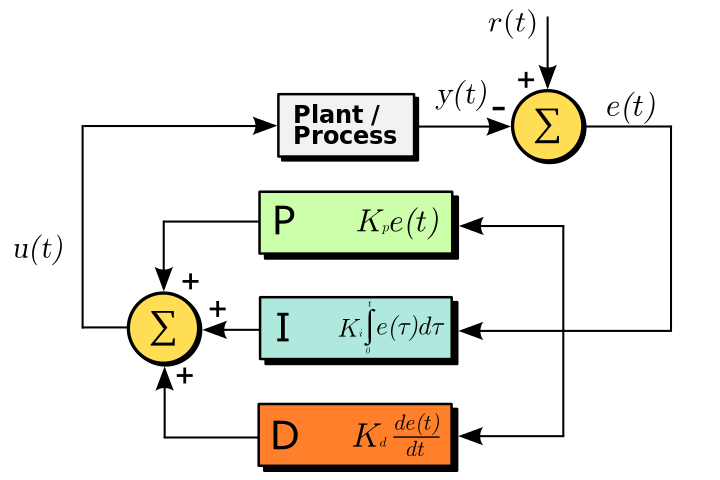
\includegraphics[width=1.0\textwidth]{figures/PID_block.png}  
\caption{Block diagram showing the PID controller} \subcaption*{Credits: \url{www.wikipedia.org/wiki/PID_controller}}  
  \label{PID controller}
\end{figure}

\newpage

\subsection {Proportional control(P)}
The proportional part creates an output value that is proportionally related to the current error value, this value can be tuned by multiplying the error by a constant $K_p$. A high proportional gain results in a large change in the output for a given change in the error. 


$$ P_{\mathrm{out}}=K_p\,{e(t)}$$  

If the proportional gain is too high, the system can become unstable. Contrarily, a small gain will result in the device adjusting too slowly, which decreases overall efficiency and in the case of this project, it will end up being detrimental to the steering accuracy.


\begin{figure}[h!]
  \centering
  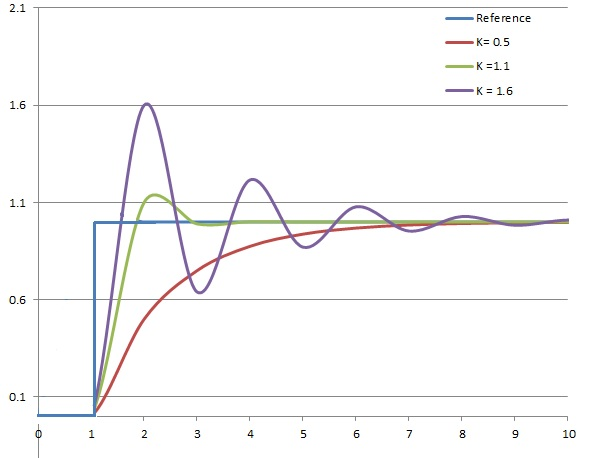
\includegraphics[width=0.8\textwidth]{figures/PIDP.jpg}
  
  \caption{$K_p$ with 3 values ($K_i$, $K_d$ held constant)} 
  \subcaption*{Credits: \url{www.wikipedia.org/wiki/PID_controller\#Proportional_term}}
  \label{PID controller}
\end{figure}


\newpage

\subsection {Integral control(I)}
The integral controller is contributing proportionally to both the magnitude of the error and the duration of the error. \\
The integral in a PID controller is the sum of the instantaneous error over time and gives the accumulated offset that should have been corrected previously. \\ 

The controller output equals the accumulated error multiplied by the integral gain(Ki)\\
$$I_{\mathrm{out}}=K_{i}\int_{0}^{t}{e(\tau)}\,{d\tau}$$ 

The integral part accelerates the movement of the process towards the reference point.
Since the integral term correlates to accumulated errors from the past, it can cause the present value to overshoot the reference value.
\begin{figure}[h!]
  \centering
  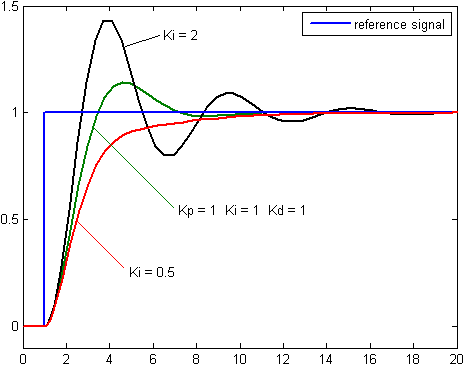
\includegraphics[width=0.8\textwidth]{figures/Change_with_Ki.png}
  
  \caption{$K_i$ shown with 3 values} 
  \subcaption*{Credits: \url{www.wikipedia.org/wiki/PID_controller\#Integral_term}}
  \label{PID controller}
\end{figure}

\newpage

\subsection {Derivative control(D)} 
The derivative of the process error is calculated by determining the slope of the error over time and multiplying this rate of change by the derivative gain $K_d$. The magnitude of the contribution of the derivative term to the overall control action is termed the derivative gain, $K_d$. The derivative term is given by:

$$D_{\mathrm{out}}=K_d\frac{de(t)}{dt}$$
The derivative action predicts system behaviour and utilizes this to improve the settling time and stability of the system.
An ideal derivative is not causal, so that implementations of PID controllers include an additional low pass filtering for the derivative term, to limit the high frequency gain and noise.
\begin{figure}[h!]
  \centering
  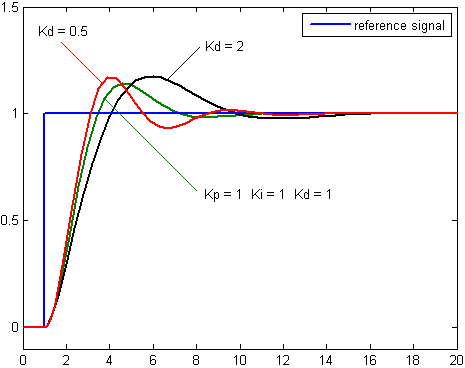
\includegraphics[width=0.8\textwidth]{figures/Change_with_Kd.png}
  \caption{$K_d$ shown with 3 values} 
  \subcaption*{Credits: \url{www.wikipedia.org/wiki/PID_controller\#Derivative_term}}
  \label{PID controller}
\end{figure}

\newpage

\subsection {Loop tuning} 
Tuning the loop is the term used to describe the adjustments of the PID’s control parameters (proportional band/gain, integral gain/reset, derivative gain/rate) to the optimal values for the given control scheme. \\ Stability is the first requirement; however systems can differ greatly, and different applications may have different requirements and these may even conflict with each other. For example, high speed and high accuracy often cancel each other out, because high speed may cause overshooting, while high accuracy is slow.\\ The ideal realistic behaviour is both as fast as possible, while also having minimum overshoot and oscillation. \\ 

Even though the process seems simple, with only three variables, it can be challenging to achieve, because it must satisfy the criteria despite being within the limitations of PID control. While adjusting the PID can seem conceptually intuitive, and while most PIDs may perform acceptably with default controls, they may very well also have an unsatisfactory performance.\\ This can generally be fixed through optimisation and tuning, either through computer simulations or manual testing.

\subsection {Steady-state error}
In figure 3.2 the reference point is the blue line. The goal is to make the lines merge up and the steady-state is achieved. When the lines don't merge and the feedback line is slightly above or under the reference point there is a steady-state error. This steady-state error can be minimized by adjusting the proportional and integral term. 


\subsection {Stability} 

If the parameters of the PID controller are set incorrectly the process input can become unstable.
This means the controllers output becomes divergent, which can be limited by saturation and mechanical breaking. \\
\newpage
\subsection {Manual tuning} 
When a system must be online at all times, a method for tuning is to first set $K_i$ and $K_d$ values to zero. Increase $K_p$ until the loop output oscillates, and then reduce $K_p$ by 10-20\%.\\
Then set $K_d$ to about 100 times the value of $K_p$ and increase or decrease until the oscillation occurs, then reduce $K_d$ by 10-20\%.\\
If needed, $K_i$ can be set to a very low number, in the case of this project, 0.01. This number is then increased or decreased, to give a fast response time without overshooting.
\\ 
A fast PID loop tuning process usually overshoots slightly to reach the reference point faster.\\ 
But in the case of systems that can't accept overshoot, an over-damped closed-loop system is best suited, which requires $K_p$ setting significantly less than half that of the $K_p$ setting that was causing the oscillation.
\\

\begin{table}[h]
\centering
\caption{Manual tuning}
\label{Table: Manual tuning}
\begin{tabular}{|l|l|l|l|l|l|}
\hline
\rowcolor[HTML]{C0C0C0} 
{\color[HTML]{000000} Parameter}                     & Rise time    & Overshoot & Settling time & Steady-state error  & Stability              \\ \hline
\cellcolor[HTML]{C0C0C0}{\color[HTML]{000000} $K_p$} & Decrease     & Increase  & Small change  & Decrease            & Degrade                \\ \hline
\cellcolor[HTML]{C0C0C0}{\color[HTML]{000000} $K_i$} & Decrease     & Increase  & Increase      & Eliminate           & Degrade                \\ \hline
\cellcolor[HTML]{C0C0C0}{\color[HTML]{000000} $K_d$} & Minor change & Decrease  & Decrease      & \begin{tabular}[c]{@{}l@{}}No effect\\ in theory\end{tabular} & \begin{tabular}[c]{@{}l@{}}Improves if\\ $K_d$ is small\end{tabular} \\ \hline
\end{tabular}
\end{table}

\subsubsection {Table \ref{Table: Manual tuning} explained}

Table \ref{Table: Manual tuning} gives an informative overview of what the different parameters does when tuned manually\footnote{http://saba.kntu.ac.ir/eecd/pcl/download/PIDtutorial.pdf}.

\begin{enumerate}
		\item[•]To minimize the rise time, decrease $K_p$
		\item[•]To eliminate the steady-state error, increase $K_i$
		\item[•]To reduce the overshoot and settling time, decrease $K_d$
	\end{enumerate}
\newpage
\subsection{PID Implementation}
In the following example, the PID constants are global variables, and therefore not part of the described function. The values are as follows: kp = 8.5, ki = 0.01, kd = 850.
\begin{lstlisting}
void PID(int sensorMean, int sensorSum)
{
	if(sensorSum > 0) //At least one sensor sees black
	{
		sensorPos = sensorMean/sensorSum; //Position of the line on the sensorarray
		sensorProp = sensorPos - 3;  //Proportional part
		sensorInt = sensorInt + sensorProp; //Integral part
		if(sensorInt > 100) //Reduce adjustment time by limiting Int
			sensorInt = 100;  
		if(sensorInt < -100)
			sensorInt = -100;
		sensorDer = sensorProp - sensorLastProp; //Derivative part
\end{lstlisting}

The PID function has two parameters, sensorMean and sensorSum. These are used to calculate where the line is in relation to the sensors. In the beginning, a check is made to make sure the line actually is on the array somewhere, since the program would stall by trying to divide by sensorSum being 0. If at least one sensor detects the line, the position is calculated by dividing the mean value of the active sensors by the amount of sensors active. Since sensorMean is calculated using weighs on each sensor, this will give the average position. The function then calculates the different parts of the PID controller, firstly the proportional part. This is done by simply subtracting the weighted value of the middle sensor from the position calculated earlier. Next up is the integral part, which is calculated by adding the previous value of the integral to the proportional value. Right after, the integral is limited since the robot will be working fast on a small line. Derivative is the last part calculated, which is done by subtracting the previous value of the proportional part from the current value.

\begin{lstlisting}
		sensorError = (sensorProp*kp)+(sensorInt*ki)+(sensorDer*kd); //PID calculation
		sensorLastProp = sensorProp; //Saves proportional for next derivative
		if(sensorError < -(initialPwm)) //Sets an upper cap for adjustment
			sensorError = -(initialPwm);
		if(sensorError > (initialPwm))
			sensorError = (initialPwm);
\end{lstlisting}
This part of the code handles the total PID value as well as limiting this value. First of all, it multiplies the previous PID values by their constants and adding these numbers together and then saves the proportional value to be handled by the derivative part next time. At the end, sensorError is limited to the maximum speed of the motors, to make future calculations easier.
\newpage
\begin{lstlisting}
		if(sensorError<0)
		{
			adjustedPWM[0] = initialPwm-sensorError; //Increase left motor, sensorError is negative here
			adjustedPWM[1] = initialPwm+sensorError; //Decrease right motor
			dir = 1; //turn right
		}
		else if(sensorError>0)
		{
			adjustedPWM[0] = initialPwm-sensorError;
			adjustedPWM[1] = initialPwm+sensorError; 
			dir = 0; //turn left
		}
		else
		{
			adjustedPWM[0] = initialPwm;
			adjustedPWM[1] = initialPwm;
			dir = 2;
		}
	}
}
\end{lstlisting}
The final part of the PID function handles the duty cycle sent to the motors. If sensorError is less than 0, the robot needs to turn right, increasing motor power on the left while decreasing motor power on the right. If sensorError is positive, do the opposite. If sensorError is exactly 0, the duty cycle will remain what it was last iteration, which is a very rare case.
\newpage
\section{Pulse-width modulation}

A pulse-width modulation technique used to encode a message into a pulsing signal. Its primary use is to control the power supply of electronic devices - the case of this project; this means the motors.\\
The average voltage and amplitude output to the motors is altered by rapidly switching between an 'on' and 'off' state.
Pulse-width modulation utilizes a square-wave signal, where the width of the pulse is modulated to get the variation in the average value of the waveform.\\ Given the pulse waveform $f(t)$ over the period $T$, low value $y_\mathrm{min}$ and high value $y_\mathrm{high}$ and duty cycle $D$, the average waveform is given by: \\

$$\overline{y}=\frac{1}{T}\int_{0}^{T}f(t)dt$$\

This expression can be simplified where $y_\mathrm{min}=0$ as $\overline{y}=D \cdot y_\mathrm{max}$. From this it can be observed that the average value of the signal $(\overline{y})$ has a direct correlation with the duty cycle D.\footnote{\url{https://en.wikipedia.org/wiki/Pulse-width_modulation\#Principle}}.
 
 $$\overline{y}=\frac{1}{T}\left(\int_{0}^{DT}y_\mathrm{max}dt+\int_{DT}^{T}y_\mathrm{min}dt\right)$$
 $$=\frac{1}{T}\left(D \cdot T \cdot y_\mathrm{max}+T(1-D)y_\mathrm{min}\right)$$
 $$=D \cdot y_\mathrm{max}+\left(1-D\right)y_\mathrm{min}$$\
  
\newpage
\subsection{Duty cycles}
The duty cycle describes the proportion of 'on' compared to any given period of runtime for the device. The duty cycle is described as a percentage, where 100\% means that it's turned on the entire time, where 10\% would be a tenth of the time.\\
$${D}=\frac{T}{P} \cdot 100\%$$ 

\begin{enumerate}
\item[•]Where {\textbf{D}} is the duty cycle. 
\item[•]{\textbf{T}} is the time the signal is active.
\item[•]{\textbf{P}} is the total period of the signal.
\end{enumerate}

\begin{figure}[h!]
  \centering
  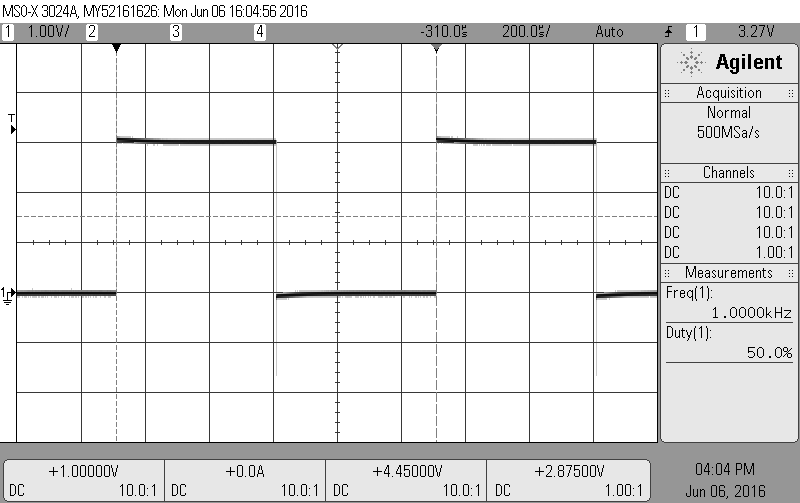
\includegraphics[width=0.7\textwidth]{figures/f1000d50.png}  
\caption{Picture of the duty cycles on an oscilloscope.}  
  \label{Duty cycles}
\end{figure}
\newpage

\section{The interface}
The project utilizes a GUI written in C\# , it shows a graphical representation of the sensor load, as well as which motor is running in accordance to the PID.\
The GUI has controls to set the COM-port as well as the baud rate, and a button prompt to connect and disconnect the robots blue-tooth transmission. It also features a terminal in the bottom, showing all the data sent from the MCU to the robot.

\begin{figure}[h!]
  \centering
  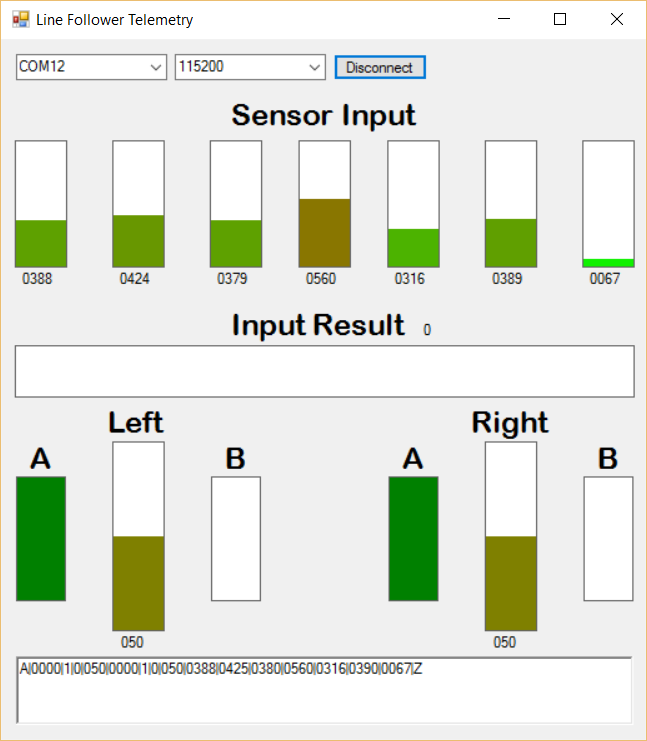
\includegraphics[width=0.5\textwidth]{figures/sensorsonwhite.png}  
\caption{Screenshot of the C\# GUI used to monitor the input readings}  
  \label{The GUI}
\end{figure}